{[}\href{terrier_desktop.html}{Previous: Desktop Search}{]}
{[}\href{index.html}{Contents}{]} {[}\href{website_search.html}{Next:
Website Search Application}{]}\\

\section{Using Terrier for Web-based
Search}\label{using-terrier-for-web-based-search}

Terrier supports dynamic search functionality in a Web browser
environment. In particular, Terrier provides a customisable Web-based
interface to facilitate retrieval of documents for a query and the
summarisation of those documents in the form of snippets or abstracts,
for display, in a similar way to major Web search engines. This page
explains how to configure Terrier to enable a Web-based search interface
like the one shown below:

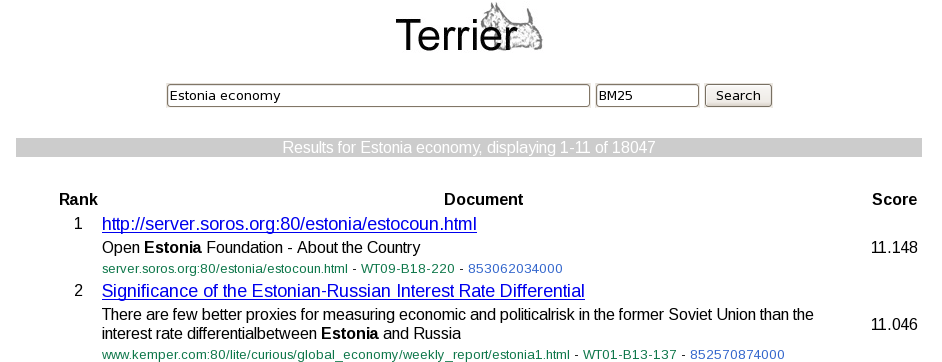
\includegraphics{images/WT2GWebInterface.png}

\subsection{Requirements}\label{requirements}

Firstly, the Web-based interface has slightly higher requirements than
Terrier -- in particular, as
\href{http://en.wikipedia.org/wiki/JavaServer_Pages}{JSPs} are used, the
full Java Development Kit (JDK) is required, instead of the JRE. To
download the JDK, see
\href{http://java.sun.com/javase/downloads/index.jsp}{Java downloads}.
Relatedly, ensure that the JAVA\_HOME environment variable points to
your JDK installation. Secondly, for existing users of Terrier, it is
important to note that normal indices cannot be used with the Web-based
interface as by default Terrier does not store document
snippets/abstracts/meta-data. Hence, the collections need to be indexed
from scratch using the correct indexing configuration.

\subsection{Indexing for a Web-based
interface}\label{indexing-for-a-web-based-interface}

As noted above, to use the Web-based interface, document
snippets/abstracts/meta-data need to be stored such that they can be
returned with each document retrieved. Normally, this will take the form
of one or more document abstracts, e.g. the first paragraph or so of
each document. The Terrier
\href{javadoc/org/terrier/indexing/Document.html}{Document} classes are
responsible for generating document abstracts. Since version 3.5, the
following Terrier classes implementing the
\href{javadoc/org/terrier/indexing/Document.html}{Document} interface
support some form of abstract generation:

\begin{itemize}
\tightlist
\item
  \href{javadoc/org/terrier/indexing/FileDocument.html}{FileDocument}:
  First \texttt{N} characters of the document.
\item
  \href{javadoc/org/terrier/indexing/POIDocument.html}{POIDocument} (for
  Microsoft Office documents, extends
  \href{javadoc/org/terrier/indexing/FileDocument.html}{FileDocument}):
  First \texttt{N} characters of the document.
\item
  \href{javadoc/org/terrier/indexing/PDFDocument.html}{PDFDocument}
  (extends
  \href{javadoc/org/terrier/indexing/FileDocument.html}{FileDocument}):
  First \texttt{N} characters of the document.
\item
  \href{javadoc/org/terrier/indexing/TaggedDocument.html}{TaggedDocument}:
  First \texttt{N} characters from the content of each specified tag
  within the document.
\item
  \href{javadoc/org/terrier/indexing/TRECDocument.html}{TRECDocument}
  (extends
  \href{javadoc/org/terrier/indexing/TaggedDocument.html}{TaggedDocument}):
  First \texttt{N} characters from the content of each specified tag
  within the document.
\end{itemize}

To configure Terrier's indexing process to store one or more document
abstracts, the appropriate properties specified in either
\href{javadoc/org/terrier/indexing/FileDocument.html}{FileDocument} or
\href{javadoc/org/terrier/indexing/TaggedDocument.html}{TaggedDocument}
must be set. Which document class to use is determined by the Collection
to be indexed. For example,
\href{javadoc/org/terrier/indexing/TRECCollection.html}{TRECCollection}
and
\href{javadoc/org/terrier/indexing/WARC018Collection.html}{WARC018Collection}
use the TaggedDocument class by default.

During indexing, Terrier stores each abstract generated as document
properties in the
\href{javadoc/org/terrier/structures/MetaIndex.html}{MetaIndex}. Note
that this can cause the MetaIndex to become quite large! To configure
this, the abstract names should be added to
\texttt{indexer.meta.forward.keys} and the abstract lengths should be
added to \texttt{indexer.meta.forward.keylens}.

An example where we save two abstracts using a TREC Collection is shown
below:

\begin{verbatim}
#For TREC collections
trec.collection.class=TRECCollection
#For ClueWeb09 collection
#trec.collection.class=WARC018Collection
#For ClueWeb12 collection
#trec.collection.class=WARC10Collection

# Do not skip any of the tags, in particular, do not skip the DOCHDR which we want to parse
# the url and crawldate from!
TrecDocTags.skip=

#TRECWebCollection uses TaggedDocument to generate abstracts
# We will save two abstracts named 'title' and 'body'
TaggedDocument.abstracts=title,body
# The tags from which to save the text. ELSE is special tag name, which means anything not consumed by other tags.
TaggedDocument.abstracts.tags=title,ELSE
# Should the tags from which we create abstracts be case-sensitive?
TaggedDocument.abstracts.tags.casesensitive=false
# The max lengths of the abstracts. Abstracts will be cropped to this length. Defaults to empty.
TaggedDocument.abstracts.lengths=256,2048

# If the document class had been a FileDocument then we would use different properties, e.g.
# FileDocument.abstract=title
# FileDocument.abstract.length=256

# We also need to tell the indexer to store the abstracts generated
# In addition to the docno, we also need to move the 'title' and 'abstract' abstracts generated to the meta index
indexer.meta.forward.keys=docno,title,abstract
# The maximum lengths for the meta index entries.
indexer.meta.forward.keylens=26,256,2048
# We will not be doing reverse lookups using the abstracts and so they are not listed here.
indexer.meta.reverse.keys=docno
\end{verbatim}

In this example, we store the first 256 characters of the title tag in
one abstract called `title' and a further 2048 characters from the rest
of the document in a second abstract called `body'. The Document class
used in this case is TaggedDocument.

\subsubsection{TRECCollection, TRECWebCollection and
Meta-Data}\label{treccollection-trecwebcollection-and-meta-data}

Beyond generating an abstract of each document, it is often useful to
store other meta-data about each document, e.g. the URL of the document
or the timestamp when the page was created, which we might also wish to
display. Importantly, this data may be held in the header of the
document or in special tags, which would otherwise be ignored by the
document parser. As such, this meta-data cannot be collected by the
document class. Instead, for collections of Web documents that have such
meta-data, the related collection class is responsible for storing this
meta-data. Currently
\href{javadoc/org/terrier/indexing/TRECCollection.html}{TRECCollection}
and
\href{javadoc/org/terrier/indexing/TRECWebCollection.html}{TRECWebCollection}
can save additional meta-data about each document as follows:

\href{javadoc/org/terrier/indexing/TRECCollection.html}{TRECCollection}
provides a simple way to directly add the content of specified document
tags to the MetaIndex. In particular, by setting
\texttt{(tagset).propertytags} -- a comma separated list of tags -- will
add those tags to the MetaIndex if they exist. Note that tags are
assumed to be IN ORDER after the docno, and that property tags are not
subsequently indexed. For example, given the following TRECDocument:

\begin{verbatim}
<DOC>
<DOCNO>Example-0001</DOCNO>
<URL>http://terrier.org</URL>
<CONTENT>The Terrier Project</CONTENT>
</DOC>
\end{verbatim}

Setting the property \texttt{TRECDocTags.propertytags=URL} will add the
contents of the URL tag to the MetaIndex with the name `URL'.

\href{javadoc/org/terrier/indexing/TRECWebCollection.html}{TRECWebCollection}
was designed to parse out additional meta-data from the header of each
document in a TRECCollection. For example, the header of a TREC WT2G
document is as follows:

\begin{verbatim}
<DOC>
<DOCNO>WT01-B01-1</DOCNO>
<DOCOLDNO>IA073-000475-B029-48</DOCOLDNO>
<DOCHDR>
http://www.city.geneva.ny.us:80/index.htm 192.108.245.124 19970121041510 text/html 2407
HTTP/1.0 200 OK
Date: Tue, 21 Jan 1997 04:14:08 GMT
Server: Apache/1.1.1
Content-type: text/html
Content-length: 2236
Last-modified: Fri, 18 Oct 1996 17:33:56 GMT
</DOCHDR>
\end{verbatim}

In particular, the TRECWebCollection class parses out the following
document meta-data where available:

\begin{itemize}
\tightlist
\item
  url (all corpora)
\item
  ip (WT2G, WT10G only)
\item
  docbytelength (WT2G, WT10G, Blogs06, Blogs08 only)
\item
  contenttype (WT2G, WT10G only, but usually identified in the HTTP
  headers)
\item
  crawldate (WT2G, WT10G only)
\end{itemize}

Note that when using these collection classes, the Terrier indexing
process needs to be told to add this additional meta-data to the
MetaIndex. As before, the meta-data names should be added to
\texttt{indexer.meta.forward.keys} and the meta-data lengths should be
added to \texttt{indexer.meta.forward.keylens}.

\subsubsection{Indexing Example: WT2G}\label{indexing-example-wt2g}

Below are the indexing properties to set when indexing the TREC WT2G
corpus such that the interface example shown earlier can be generated.
Note that these properties should be used \emph{in addition to} the
standard \href{configure_indexing.html}{indexing} and
\href{configure_retrieval.html}{retrieval} properties.

\begin{verbatim}
# WT2G is a TRECCollection and we want to get the crawldate and urls from the header
# hence we use TRECWebCollection. No additional properties are needed as TRECWebCollection
# extracts the data by default
trec.collection.class=TRECWebCollection

# Do not skip any of the tags, in particular, do not skip the DOCHDR which we want to parse
# the url and crawldate from!
TrecDocTags.skip=

#TRECWebCollection uses TaggedDocument to generate abstracts
# We will save two abstracts called 'title' and 'body'
TaggedDocument.abstracts=title,body
# We create abstracts from the title tag and the rest each document (ELSE).
TaggedDocument.abstracts.tags=title,ELSE
# Should the tags from which we create abstracts be case-sensitive?
TaggedDocument.abstracts.tags.casesensitive=false
# The max lengths of the abstracts. 256 for the title, 2048 for the body.
TaggedDocument.abstracts.lengths=256,2048

# We also need to tell the indexer to store the abstracts generated from TaggedDocument and
# the crawldate/urls saved by TRECWebCollection
# In addition to the docno which we always have, we also need tell the indexer to store the
# 'title' and 'body'  abstracts generated, in addition to the url and crawldate extracted in the
# meta index
indexer.meta.forward.keys=docno,title,body,url,crawldate
# The maximum lengths for the meta index entries.
indexer.meta.forward.keylens=32,256,2048,200,35
# We will not be doing reverse lookups using the abstracts and so they are not listed here.
indexer.meta.reverse.keys=docno
\end{verbatim}

\subsection{Using the Web-based
interface}\label{using-the-web-based-interface}

Once you have an index with the necessary abstract entries and/or
meta-data, you can start a Web-based interface, and begin searching with
it. We provide two basic interfaces for illustration, `simple' and
`wt2g'. These are stored in: \texttt{src/webapps/}. By default, the
`simple' interface can be launched using the following command:

\begin{verbatim}
bin/http_terrier.sh
\end{verbatim}

This will start a local HTTP server hosting the src/webapps/simple
folder at :

\begin{verbatim}
http://localhost:8080/
\end{verbatim}

Below is an example of a the top search result returned using the
`simple' interface for the query `Estonia economy' when searching the
WT2G collection using BM25. The simple interface lists all stored meta
entries for each of the retrieved documents, including the docno, title
and url.

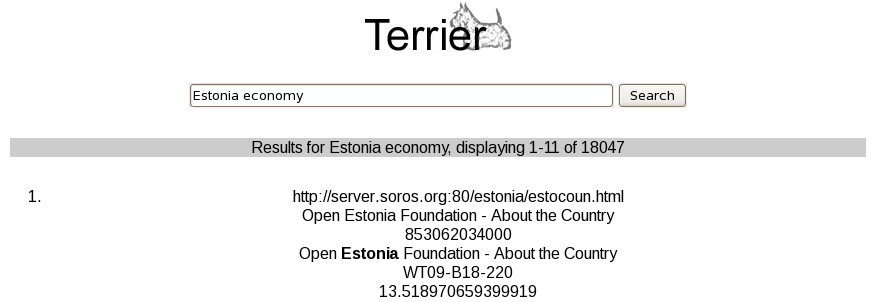
\includegraphics{images/SimpleWebInterface.png}

This interface is a
\href{http://en.wikipedia.org/wiki/JavaServer_Pages}{JSP} file stored at
\texttt{src/webapps/simple/results.jsp}. When it is called, it opens the
Terrier index specified in the terrier.properties file (if not already
open), initialises a manager and retrieves the results for the specified
query as a standard terrier ResultSet just like the normal Java
application. Of importance is that Terrier must be instructed to
decorate the ResultSet with all of the meta-data that we stored
previously such that results.jsp can display it. This is done as a
Terrier \href{javadoc/org/terrier/querying/PostFilter.html}{PostFilter},
in particular using either the
\href{javadoc/org/terrier/querying/SimpleDecorate.html}{SimpleDecorate}
or \href{javadoc/org/terrier/querying/Decorate.html}{Decorate} classes.
SimpleDecorate adds all meta index entries for each document retrieved
into the ResultSet. Decorate is more advanced, providing query text
highlighting and query-biased summarisation. Below we provide an example
where we decorate the Result set using the more advanced Decorate class
in the terrier.properties file:

\begin{verbatim}
# We are using org.terrier.querying.Decorate which we are going to name decorate (IMPORTANT: results.jsp
# expects it to be called 'decorate')
querying.postfilters.controls=decorate:org.terrier.querying.Decorate
# In what order should we process the filters? (we have only one so this does nothing but is required)
querying.postfilters.order=org.terrier.querying.Decorate

#default and allowed controls
# decorate:on - activate the decorate process
# summaries:body - special control for the org.terrier.querying.Decorate class, tells it to create a
#                  query-biased summary based on the text stored in the abstract named 'body'
# emphasis:title;body - special control for the org.terrier.querying.Decorate class, tells it to create
#                       additional meta-data where the query terms are emphasised. These are named
#                       _emph, where name is the meta entry name. In this case, we create two new
#                       entries called title_emph and body_emph based on the title and body abstracts. 
querying.default.controls=decorate:on,summaries:body,emphasis:title;body
# We need to also state that decorate is an allowed control
querying.allowed.controls=c,scope,decorate,start,end
\end{verbatim}

\subsubsection{Customising look \& feel}\label{customising-look-feel}

The simple interface provides only the basic functionality. You can
change the look and feel of the search results by editing
src/webapps/simple/results.jsp, or the stylesheet in the same location.
Changes made to results.jsp should have an immediate effect on the
results. We provide a second example interface designed to display
documents from WT2G, named wt2g (\texttt{src/webapps/wt2g/})

If you wish to use another webapps folder, or start the interface on a
port other than 8080, you can override both on the command line.

\begin{verbatim}
bin/http_terrier.sh 8080 src/webapps/wt2g/
\end{verbatim}

The results for the same example query using the wt2g interface are
shown below.

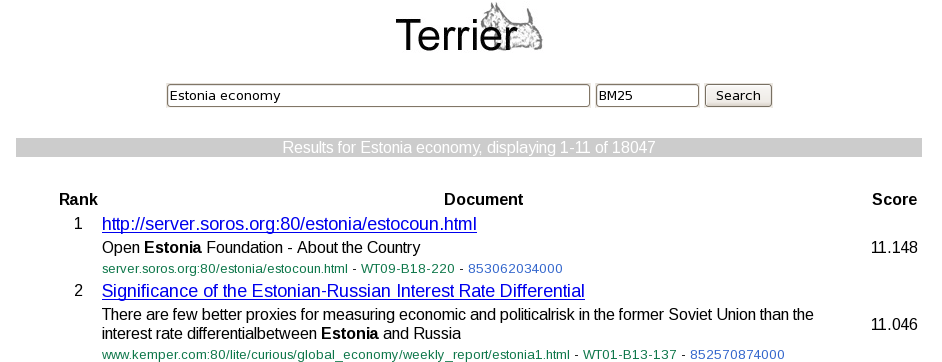
\includegraphics{images/WT2GWebInterface.png}

\subsubsection{Extending the Query
Language}\label{extending-the-query-language}

Terrier provides several
\href{javadoc/org/terrier/querying/PostFilter.html}{PostFilters} that
are useful for interactive operation. For example, the
\href{javadoc/org/terrier/querying/SiteFilter.html}{SiteFilter} is an
implementation of the \texttt{site:} control from standard Web search
engines, and ensures that returned results have a hostname matching the
desired expression. The hostname is obtained from the \texttt{url}
metadata from the MetaIndex. For example, adding \texttt{site:com} to
the query will ensure that all results have URLs from the .com domain.
For TREC or similar collections, the
\href{javadoc/org/terrier/querying/Scope.html}{Scope} filter permits a
starting prefix on the docno document metadata from the MetaIndex.

\subsubsection{Extending Results.jsp}\label{extending-results.jsp}

The two initial interfaces provided with Terrier can be easily extended
to add more control when searching or to add new functionality. Below we
provide a commented extract from results.jsp that covers the retrieval
component of the interface.

\begin{verbatim}
// Get the index if already stored in terrier.jsp.index or load a new one
Index index = (Index)application.getAttribute("terrier.jsp.index");
if (index == null)
{
    index = Index.createIndex();
    application.setAttribute("terrier.jsp.index", index);
}

// Initialise the manager which controls the querying process   
Manager queryingManager = (Manager)application.getAttribute("terrier.jsp.manager");
if (queryingManager == null)
{
    queryingManager = new Manager(index);
    application.setAttribute("terrier.jsp.manager", queryingManager);
}

// Make a new search request with the query ('query' is parsed from the HTML form earlier)
SearchRequest srq = queryingManager.newSearchRequest("results.jsp.query", query);
srq.setOriginalQuery(query);

// Are we starting at rank 1? We could be on page 1 or 2 of the results, where sStart would
// be 11 or 21 respectively (ten per page)
srq.setControl("start", sStart);

// This actives the 'decorate' post process that adds all of the meta entries for each document
// to the ResultSet such that this jsp can display them
srq.setControl("decorate", "on");

// Extra controls could be added here, for example query expansion or site filtering
// The appropriate properties in terrier.properties need to be set and then the post process
// activated if requested in the html form, e.g. assuming there is a field called doQueryExpansion:
// String doQueryExpansion = request.getParameter("doQueryExpansion");
// if (doQueryExpansion == null || doQueryExpansion.length() == 0)
//  doQueryExpansion=null;
// doQueryExpansion = doQueryExpansion.trim();
// if ( doQueryExpansion!=null ) srq.setControl("qe", "on");

// The last document to return
srq.setControl("end", String.valueOf(iStart + NUM_RESULTS_PER_PAGE -1));
// The matching model to choose
srq.addMatchingModel(defaultMatching, defaultModel);
// Run any preprocessing (e.g. run the query through the term pipeline)
queryingManager.runPreProcessing(srq);
// Get the documents that match the query)
queryingManager.runMatching(srq);
// Run any postprocessing - (e.g. query expansion)
queryingManager.runPostProcessing(srq);
// Run any postfilters - at this stage the 'decorate' post filter adds the meta-data about each
// document to the ResultSet
queryingManager.runPostFilters(srq);
// Get our decorated result set
ResultSet rs = srq.getResultSet();
\end{verbatim}

\subsubsection{Further Details}\label{further-details}

\texttt{bin/http\_terrier.sh} invokes
\href{javadoc/org/terrier/utility/SimpleJettyHTTPServer.html}{SimpleJettyHTTPServer},
which starts a \href{http://www.eclipse.org/jetty/}{Jetty} server on the
port specified on the command line. The second command line argument is
the path to a webapps folder. \texttt{share/images} is also mounted as
\texttt{/images} directory.

{[}\href{terrier_desktop.html}{Previous: Desktop Search}{]}
{[}\href{index.html}{Contents}{]} {[}\href{website_search.html}{Next:
Website Search Application}{]}

\begin{center}\rule{0.5\linewidth}{\linethickness}\end{center}

Webpage: \url{http://terrier.org}\\
Contact:
\href{mailto:terrier@dcs.gla.ac.uk}{\nolinkurl{terrier@dcs.gla.ac.uk}}\\
\href{http://www.dcs.gla.ac.uk/}{School of Computing Science}\\
Copyright (C) 2004-2015 \href{http://www.gla.ac.uk/}{University of
Glasgow}. All Rights Reserved.

~
